\documentclass{article}  % Define la clase del documento.

% Paquetes de idioma y codificación
\usepackage[utf8]{inputenc}
\usepackage[T1]{fontenc}
\usepackage[spanish]{babel}  % Ajusta el idioma del documento a español.
\usepackage{tabularx}  % Permite la creación de tablas con ancho ajustable.

% Paquete de geometría para configurar márgenes y tamaño de papel
\usepackage[letterpaper, margin=3cm]{geometry}

% Paquetes de tipografía
\usepackage{mathptmx}    % Usa Times New Roman como fuente.
\usepackage{microtype}   % Mejora la justificación del texto.

% Paquetes para manejo de colores y gráficos
\usepackage{xcolor}      % Define y utiliza colores.
\usepackage{graphicx}    % Permite la inserción de imágenes.
\usepackage{tikz}        % Creación de gráficos vectoriales.

% Configuración de enlaces y referencias cruzadas
\usepackage{hyperref}
\hypersetup{
    colorlinks   = true,
    linkcolor    = darkblue,
    citecolor    = black,
    filecolor    = blue,
    urlcolor     = blue
}

%\usepackage{etoolbox}  % Carga este paquete en el preámbulo para modificar entornos de bibliografia
%\patchcmd{\thebibliography}{\chapter*}{\part*}{}{}

\usepackage{media9} % Permite la inserción de multimedia.

% Paquetes para la mejora visual de tablas y figuras
\usepackage{booktabs}    % Para tablas de alta calidad.
\usepackage{float}       % Controla la posición de figuras y tablas.

% Paquete para la personalización de códigos fuente
\usepackage{listings}
\lstset{
    literate=
    {á}{{\'a}}1 {é}{{\'e}}1 {í}{{\'i}}1 {ó}{{\'o}}1 {ú}{{\'u}}1
    {Á}{{\'A}}1 {É}{{\'E}}1 {Í}{{\'I}}1 {Ó}{{\'O}}1 {Ú}{{\'U}}1
    {ñ}{{\~n}}1 {Ñ}{{\~N}}1 {ü}{{\"u}}1 {Ü}{{\"U}}1,
    backgroundcolor=\color{backcolour},
    commentstyle=\color{codegreen},
    keywordstyle=\color{codepurple},
    numberstyle=\tiny\color{codegray},
    stringstyle=\color{red},
    basicstyle=\ttfamily\small,
    breakatwhitespace=false,
    breaklines=true,
    captionpos=b,
    keepspaces=true,
    numbers=left,
    numbersep=5pt,
    showspaces=false,
    showstringspaces=false,
    showtabs=false,
    tabsize=2,
    language=TeX,
    morecomment=[l]\#,
    frame=single,
    rulecolor=\color{black}
}

% Definición de colores al estilo Visual Studio Code
\definecolor{darkblue}{rgb}{0.0, 0.0, 0.55}  % Enlaces
\definecolor{codegreen}{rgb}{0.25, 0.49, 0.48}  % Comentarios
\definecolor{codegray}{rgb}{0.5, 0.5, 0.5}  % Números y anotaciones
\definecolor{codepurple}{rgb}{0.58, 0, 0.82}  % Palabras clave
\definecolor{backcolour}{rgb}{0.95, 0.95, 0.92}  % Fondo de código

% Configuraciones de párrafo y matemáticas
\usepackage{amsmath}
\usepackage{parskip}    % Espaciado entre párrafos.
\usepackage{ragged2e}   % Justificación mejorada.

% Configuración de secciones y encabezados
\usepackage{titlesec}
\titleclass{\part}{top} % Make part like a class
\titleformat{\part}[display]
  {\normalfont\huge\bfseries\centering}{\thepart}{40pt}{\Huge}
\titlespacing*{\part}{0pt}{-60pt}{10pt}
\titleformat{\part}
  {\normalfont\huge\bfseries}{}{0pt}{}

% Asegúrate de usar esto para mantener el estilo en las páginas de las partes
\titleformat{\part}[display]
  {\normalfont\huge\bfseries}{}{0pt}{}
  [\thispagestyle{fancy}] % Aplica el estilo fancy a las páginas de las partes

% Configuración de encabezados y pies de página personalizados
\usepackage{fancyhdr}
\pagestyle{fancy}
\fancyhf{}
\fancyhead[L]{\raisebox{0.20cm}{\textbf{Métodos Computacionales en Obras Civiles}}}
\fancyhead[R]{\raisebox{0.1cm}{
\includegraphics[width=0.25\linewidth]{LOGO_UNIVERSIDAD.jpg}}}
\fancyhead[C]{\rule{\textwidth}{0.6pt}}
\fancyfoot[C]{\rule{\textwidth}{0.6pt}}
\fancyfoot[R]{\raisebox{-1.5\baselineskip}{\thepage}}
\renewcommand{\headrulewidth}{0pt}
\renewcommand{\footrulewidth}{0pt}

% Configuración avanzada de geometría
\geometry{
  top=3.5cm, % Aumenta el espacio en la parte superior para subir el encabezado
  bottom=2.5cm,
  headheight=2.5cm % Aumenta la altura del encabezado si es necesario
}

% Configuracion de bibliografia
\usepackage{natbib}
\bibliographystyle{unsrtnat}  % Puedes cambiarlo por `unsrtnat`, `abbrvnat`, etc.
\usepackage{tabularx} 
\begin{document}
%----------------------------------------------------------------------------------------
% PORTADA
%----------------------------------------------------------------------------------------
\begin{titlepage}%Inicio de la carátula, solo modificar los datos necesarios
\newcommand{\HRule}{\rule{\linewidth}{0.5mm}} 
\center 
%----------------------------------------------------------------------------------------
%	ENCABEZADO
%----------------------------------------------------------------------------------------

\includegraphics[width=10cm]{LOGO_UNIVERSIDAD.jpg}\\ % Si esta plantilla se copio correctamente, va a llevar la imagen del logo de la facultad.OBS: Es necesario incluir el paquete: graphicx
\vspace{3cm}
%----------------------------------------------------------------------------------------
%	SECCION DEL TITULO
%----------------------------------------------------------------------------------------
\HRule \\[0.4cm]
{ \huge \bfseries Entrega 3, Proyecto 1}\\[0.4cm] % Titulo del documento
{ \huge \bfseries Metodos Computacionales en OOCC, IOC 4201}\\[0.4cm] % Titulo del documento
\HRule \\[1.5cm]
 \vspace{4.5cm}
%----------------------------------------------------------------------------------------
%	SECCION DEL AUTOR
%----------------------------------------------------------------------------------------
\begin{flushright}
    { \textbf{Profesor:}\\
    Patricio Moreno\\
    \vspace{0.2cm}
    \textbf{Ayudante:} \\
    Maximiliano Biasi\\
    \vspace{0.2cm}
    \textbf{Alumno:} \\
    Bernardo Caprile Canala-Echevarría\\
    Pedro Tomás Valenzuela Bejares\\
    Felipe Alberto Vicencio Fossa\\
    Lukas Wolff Casanova\\
}
\end{flushright}
\vspace{1cm}
%----------------------------------------------------------------------------------------
%	SECCION DE LA FECHA
%----------------------------------------------------------------------------------------
{\large \textbf{\today}}\\[2cm] % El comando \today coloca la fecha del dia, y esto se actualiza con cada compilacion, en caso de querer tener una fecha estatica, reemplazar el \today por la fecha deseada
\end{titlepage}
%----------------------------------------------------------------------------------------
%  INDICE
%----------------------------------------------------------------------------------------
\newpage
\thispagestyle{empty} % Deshabilita el número de página en la página del índice
\tableofcontents
\thispagestyle{plain} % Deshabilita el encabezado en la página del índice
\thispagestyle{empty} % Deshabilita el número de página en la página del índice

\thispagestyle{empty}
\listoffigures 
\thispagestyle{plain} % Deshabilita el encabezado en la página del índice %
\thispagestyle{empty}
\newpage
%----------------------------------------------------------------------------------------
%ACÁ EMPIEZA EL INFORME
\setcounter{page}{1}
%----------------------------------------------------------------------------------------

\part{Entrega 0}

\section{Comandos Para Correr Arquitectura X86 en Arquitectura ARM}

Debido a que trabajo en MAC, la arquitectura utilizadas es ARM 64, donde el requerimiento para las librerias es X86, por lo que se debe correr una instancia de X86 en la arquitectura ARM, donde para activar el entorno, se utilizan los siguientes comandos:

Primero se llama la instancia en una arquitectura X86

\begin{verbatim}
    arch -x86_64 python3 -m venv x86_env
\end{verbatim}

Luego se activa

\begin{verbatim}
    source x86_env/bin/activate
\end{verbatim}

Para instalar las librerias necesarias

\begin{verbatim}
    arch -x86_64 pip install <librerias>
\end{verbatim}

Finalmente debo correr el codigo desde la instancia

\begin{verbatim}
    arch -x86_64 python3 <ruta> .py
\end{verbatim}


\section{Calculos Manuales}

\subsection{Claculo de alturas}

Para calcular la altura de los puntos desconocidos, se determino el momento en tal nodo, obteniendo asi:

\begin{table}[H]
    \centering
    \begin{tabular}{|c|c|}
    \hline
    \textbf{Nodo} & \textbf{Altura [m]}  \\ 
    \hline
    B & 7.733  \\ 
    C & 11.733  \\ 
    E & 9.400 \\ 
    \hline
    \end{tabular}
    \caption{LAturas Nodos Desconocidos}
\end{table}

\subsection{Solucion Reticulado}

El codigo realizado para calcular el reticulado se encuentra en el \href{https://github.com/LukasWolff2002/PROYECTO_3_MCOC/blob/main/CODIGO/CODIGO_MANUAL/solucion_reticulado.py}{siguiente link}, donde, para calcular la seccion de las barras, se utilizo el \href{https://github.com/LukasWolff2002/PROYECTO_3_MCOC/blob/main/CODIGO/CODIGO_MANUAL/tipo_barras.py}{siguiente codigo}.

\begin{table}[H]
    \centering
    \begin{tabular}{|c|c|c|c|c|}
    \hline
    \textbf{Barra} & \textbf{Esfuerzo Interno} & \textbf{D$_{int}$, D$_{ext}$ [mm]} & \textbf{Tensiones Internas} & \textbf{Fuerza Critica Pandeo} \\ 
    \hline
    AB & 89.411 & (117.000, 135.500) & 24.371 & 117.169 \\ 
    AL & 15.000 & (85.000, 95.000) & 10.610 & 19.682 \\ 
    LK & 0.000 & (10.000, 20.000) & 0.000 & 0.227 \\ 
    LB & 0.000 & (10.000, 20.000) & 0.000 & 0.177 \\ 
    BC & 71.874 & (98.500, 114.500) & 26.852 & 94.163 \\ 
    BK & 30.000 & (52.000, 62.000) & 33.506 & 39.731 \\ 
    KJ & 0.000 & (10.000, 20.000) & 0.000 & 0.227 \\ 
    JC & 30.000 & (10.000, 20.000) & 127.324 & 204.387 \\ 
    JI & 0.000 & (10.000, 20.000) & 0.000 & 0.227 \\ 
    CI & 64.321 & (90.000, 105.000) & 27.999 & 84.599 \\ 
    IH & 0.000 & (10.000, 20.000) & 0.000 & 0.404 \\ 
    IE & 70.062 & (77.500, 93.500) & 32.604 & 91.438 \\ 
    HE & 30.000 & (36.000, 46.000) & 46.582 & 40.103 \\ 
    HG & 0.000 & (10.000, 20.000) & 0.000 & 0.404 \\ 
    GE & 0.000 & (10.000, 20.000) & 0.000 & 0.340 \\ 
    GF & 15.000 & (63.500, 73.500) & 13.941 & 19.569 \\ 
    EF & 86.488 & (92.500, 110.500) & 30.137 & 112.836 \\ 
    \hline
    \end{tabular}
    \caption{Informacion Barras}
\end{table}

\textbf{Nota:} todas las barras se encuentran en esfuerzo de comprecion.

\begin{table}[H]
\centering
\begin{tabular}{|c|c|c|}
\hline
\textbf{Key} & \textbf{FS Fluencia} & \textbf{FS Pandeo} \\ 
\hline
AB & 8.617 & 1.310 \\ 
AL & 19.792 & 1.312 \\ 
BC & 7.821 & 1.310 \\ 
BK & 6.267 & 1.324 \\ 
JC & 1.649 & 6.813 \\ 
CI & 7.500 & 1.315 \\ 
IE & 6.441 & 1.305 \\ 
HE & 4.508 & 1.337 \\ 
GF & 15.064 & 1.305 \\ 
EF & 6.968 & 1.305 \\ 
\hline
\end{tabular}
\caption{Factor de Seguridad Fluencia y Pandeo}
\end{table}

\textbf{Nota:} solo se consideran las barras que tienen algun esfuerzo interno significante para el calculo del FS.


\subsection{Calculo de Deformacion}

Para el calculo de la deformacion en el nodo D/I, se impone una fuerza virtual igual a 1, de esta manera es posible calcular el reticulado. Con todos los esfuerzos conocidos, se aplica la siguiente formula:

\begin{equation}
    \delta = \sum   \frac{P_r \cdot P_v \cdot L}{E\cdot A}
\end{equation}

Se obtuvieron los siguientes desplazamientos, donde la seccion considerada es (117, 135.5):

\begin{equation}
    \delta_x = -8.47300012321403 mm \quad \delta_y = -10.1170948633426 mm
\end{equation}

\section{Opensees}

EL codigo utilizado para hacer el modelo en Opensees se encuentra en el \href{https://github.com/LukasWolff2002/PROYECTO_3_MCOC/blob/main/CODIGO/OPENSEES/E0_Wolff.py}{siguiente link}, donde los esfuerzos obtenidos son los siguientes:

\begin{table}[H]
    \centering
    \caption{Esfuerzos internos en las barras (fuerzas axiales)}
    \label{tab:esfuerzos_internos}
    \begin{tabular}{|c|c|}
        \hline
        \textbf{Barra} & \textbf{Fuerza Axial (KN)} \\
        \hline
        AL & 15.03 \\
        AB & 89.39 \\
        LB & 0.06  \\
        LK & 0.05  \\
        KB & 30.03 \\
        BC & 71.82 \\
        KJ & 0.79  \\
        KC & 0.74  \\
        JC & 30.00 \\
        CD & 63.53 \\
        JI & 0.79  \\
        IH & 0.00  \\
        IE & 70.06 \\
        HE & 30.00 \\
        EF & 0.00  \\
        HG & 0.00  \\
        EF & 86.49 \\
        GF & 15.00 \\ \hline
    \end{tabular}
\end{table}

\textbf{Nota:} Se observa claramente una relacion directa con los resultados manuales, donde la pequeña variacion nace de la adicion de la barra \textbf{KC}.

\subsection{Deformaciones}

Para el calculo de las deformaciones, se asume una seccion igual para todas las barras, donde, segun los datosa calculados manualmente, la seccion nesesaria es (117, 135.5), los resultados obtenidos son los siguientes:

\begin{figure}[H]
    \centering
    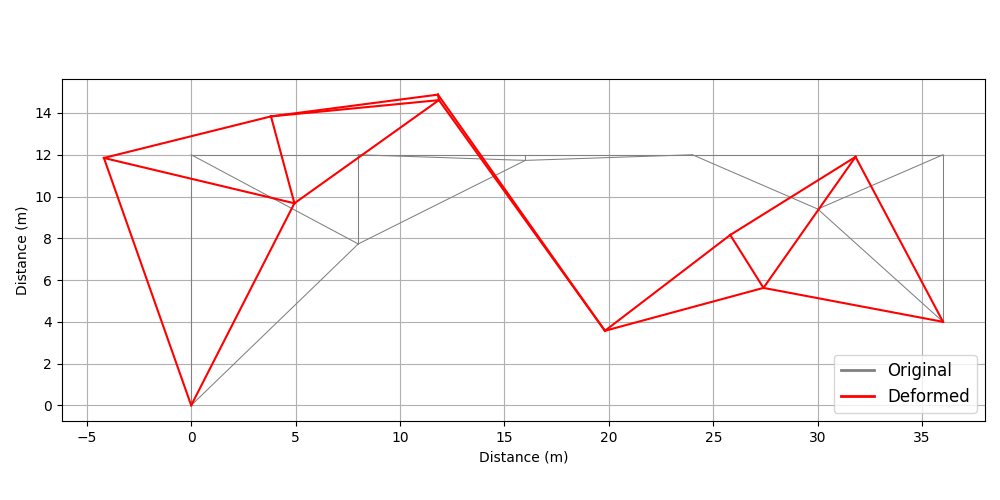
\includegraphics[width=0.8\textwidth]{GRAFICOS/deformed_truss.png}
    \caption{Deformaciones en los nodos}
    \label{fig:deformaciones}
\end{figure}

El diagrama tridimencional solicitado es el siguiente:

\begin{figure}[H]
    \centering
    \includegraphics[width=0.8\textwidth]{GRAFICOS/3D.png}
    \caption{Grafico 3D}
    \label{fig:deformaciones_3D}
\end{figure}

La deformacion observada en el nodo D/I es:

\begin{equation}
    \delta_x = -0.0065527383052691 m \quad \delta_y = -0.013182996668814742 m
\end{equation}

De esta manera, los porcentajes de error respecto al calculo manual son:

\begin{equation}
    \delta_x = 29.31\% \quad \delta_y = 30.23\%
\end{equation}





\renewcommand{\refname}{}  % Para documentos tipo 'article'
\renewcommand{\bibname}{}  % Para documentos tipo 'book' o 'report'
\newpage
\part{Referencias}  % Título de la bibliografía como un \part
\vspace{-1cm}
\bibliography{referencias}  % Nombre del archivo .bib

\end{document}
